% rubber : module pdftex
\documentclass[conference]{IEEEtran}

\usepackage{algorithm}
\usepackage{algorithmic}
\usepackage{hyphenat}
\usepackage{xspace}
\usepackage{float} \floatstyle{ruled} \restylefloat{figure} \restylefloat{table}
\usepackage{listings}
\lstset{basicstyle=\sffamily\small,showstringspaces=false,columns=fullflexible,}

\usepackage[square,sort&compress,numbers]{natbib}
\usepackage{tikz}
\usetikzlibrary{shapes,arrows}

\usepackage{graphicx}
\DeclareGraphicsExtensions{.pdf,.jpeg,.png}

\usepackage{xcolor}
\definecolor{darkblue}{rgb}{0.0, 0.18, 0.39}
\definecolor{darkgreen}{rgb}{0.18, 0.31, 0.31}
\definecolor{light-gray}{gray}{0.75}

\usepackage[pdftex]{hyperref}
\hypersetup{
    letterpaper=true,
    pagebackref=false,      % links back from references to body text
    plainpages=false,       % needed if Roman numbers in frontpages
    pdfpagelabels=true,     % adds page number as label in Acrobat's page count
    bookmarks=true,         % show bookmarks bar?
    unicode=false,          % non-Latin characters in Acrobat's bookmarks
    pdftoolbar=true,        % show Acrobat's toolbar?
    pdfmenubar=true,        % show Acrobat's menu?
    pdffitwindow=false,     % window fit to page when opened
    pdfstartview={FitH},    % fits the width of the page to the window
    pdfnewwindow=true,      % links in new window
    colorlinks=true,        % false: boxed links; true: colored links
    linkcolor=darkblue,     % color of internal links
    citecolor=darkgreen,    % color of links to bibliography
    filecolor=magenta,      % color of file links
    urlcolor=blue           % color of external links
}
\hypersetup{	% override some previously defined hyperref options
%%    colorlinks,%
    citecolor=black,%
    filecolor=black,%
    linkcolor=black,%
    urlcolor=black
}

\lstdefinelanguage{manifold}
{
  morekeywords={
    primitive,
    port,
    node,
    infer,
    public,
    import,
    Type,
    true,
    false
  },
  morecomment=[l]{//},
  morecomment=[s]{/*}{*/},
  morestring=[b]"
}

\lstset{
  language={manifold},
  basicstyle=\small\ttfamily,
  captionpos=b,
  tabsize=2,
  columns=fixed,
  keepspaces=true,
  showstringspaces=false,
  breaklines=true,
  frame=single,
  numberstyle=\tiny\ttfamily,
  commentstyle=\textit,
  keywordstyle=\textbf
}


%%%%%%%%%%%%%%%%%%%%%%%%%%%%%%%%%%%%%%%%%%%%%%%%%%%%%%%%%%%%%%%%%%%%%%%%
\begin{document}

\title{Manifold 2.0 \\ \vspace{-1ex} {\Large A Hardware Description Language for Microfluidic Devices}}
\author{\IEEEauthorblockN{Nicholas Klassen, Michael Lyons, Michael Prysiazny, 
Paul Roth, Peter Socha, \\
Murphy Berzish, Atulan Zaman, and Derek Rayside}
\IEEEauthorblockA{Electrical and Computer Engineering\\
University of Waterloo, Canada\\
\url{drayside@uwaterloo.ca}}
}

\maketitle

\begin{abstract}
We are describing our most recent progress on the Manifold systems design language and toolchain.
Manifold is a generic high-level system design language built to resemble modern functional programming languages.
It has been applied in the past to describe digital and microfluidic circuits, with most recent work focusing on microfluidics.
The Manifold toolchain allows engineers to describe their systems in a simple and high-level abstraction using domain specific libraries.
The syntax of the frontend language has been expanded with several useful features, including a type system, importable modules, functions, and tuples.
For the domain-specific microfludics backend, the framework now supports code generation for Modelica modeling language for running time-domain simulations.
By integrating with tools such as the dReal satisfiability solver Manifold allows the design verification process to be automated.
We also demonstrate the process for Manifold code input to be synthesized into schematics for MapleSim for simulation and possibly for additional tools in the future.
\end{abstract}
\begin{IEEEkeywords}
Microfluidics, Design automation, Hardware description language.
\end{IEEEkeywords}

\section{Introduction}

The field of microfluidic device engineering currently suffers from a lack of accessible tools for circuit design and analysis.
Engineers currently need to develop systems of equations that represent their circuits by hand \cite{Thorsen02science}.
One must then manually solve these equations to determine the system's viability. This is often limiting because computation time for simulating each component is significant using techniques such as finite element analysis, which limits the scalability of designs. Since there are often complex components involved in a microfluidic circuit, better computer aided design tools are required to simulate and verify the systemic behavior of connected components to allow rapid prototyping of designs.
With Manifold, engineers can describe their complete microfluidic systems in a functional programming style. 
Manifold converts this system code into inputs for third-party solver tools, which can then perform an analysis of the system described in the code.
The Manifold framework was first introduced by Berzish et. al in \cite{Berzish16cascon}.
This work follows up on the recent features that have been added to the toolchain.

The Manifold toolchain begins with a high-level hardware description language.
The engineer writes code in the Manifold frontend language to describe the desired system.
The frontend language is domain-agnostic and does not make any domain-related assumptions.
When describing a system in the frontend language, an engineer may choose to omit certain parameters of their design to have them inferred by Manifold later on in the toolchain.
The Manifold frontend compiler processes the frontend code to create an intermediate schematic.
Like the frontend language, the schematic format is generic by design, expressing all systems in terms of nodes, ports, connections, constraints, and attributes.
When needed, domain-specific parameters can be specified in the frontend language and will be written into the schematic as object attributes.

All domain-specific processing occurs in a Manifold backend compiler, which takes a schematic as input and produces domain-specific output.
Two backend compilers currently exist for Manifold: a digital circuit backend that generates VHDL code, and a microfluidics backend that generates SMT2 and Modelica code.
All of our recent work has been on the microfluidics backend.
The goal of the microfluidics backend is to generate code for multiple third-party solver tools.
Code generation in the SMT2 format and integration with the dReal satisfiability solver \cite{Gao13dReal} have long been supported features.
Code generation in Modelica for use by the MapleSim simulator is a recently-added feature.

Manifold's goal is to automate much of the design process, in particular reducing the need for manual mathematical modeling and guess-and-check work.
Instead of writing out systems equations by hand, Manifold allows engineers to write high-level system descriptions using the frontend language.
The Manifold microfluidics toolchain automatically generates relevant system equations and allows engineers to easily leverage third-party analysis tools.
The aim is to allow engineers to verify their designs quickly so that they may iterate more efficiently.

\section{The Manifold High-Level Language}

\subsection{Module System}

We created a basic module system for Manifold that will facilitate the
distribution of programming libraries to our users. The libraries that will be
provided by Manifold will expose an API for interacting with the backend
microfluidics libraries. This is similar to how programmers can define
\texttt{extern} functions in C. The Manifold libraries will define primitive
nodes that the backend will later recognize as components. These basic
components would be very difficult or impossible to represent in Manifold, so
instead we simply define an interface for the backend library. Creating
modules in Manifold also allow researchers to share their designs and have
others build on them.

Manifold's module system is as simplistic as possible, slightly more
sophisticated than including files verbatim like C's preprocessor does.
The module system is similar to the one outlined in Cardelli
\cite{Cardelli:1997:PFL:263699.263735}. Each module, in this case a file, can
declare functions and values as \texttt{public}. When a module imports another
module, all of the values in the imported module marked as public will be
accessible (Figure~\ref{lst:exports}).

\begin{lstlisting}[label=lst:exports, caption=Exported values in a Manifold file]
public digitalIn = primitive port Bool;
public digitalOut = primitive port Bool;

public inputPin = primitive node (Nil) -> (out: digitalIn);
public outputPin = primitive node (in: digitalOut) -> (Nil);

public (x, y) = (inputPin(), inputPin());

// Not exported
hiddenVar = 2
\end{lstlisting}

Manifold does not compile modules separately, and types defined in modules are
added to the global namespace when they are imported. Values from the imported
module however, are namespaced. Manifold interprets imports as expressions,
like all language constructs. Imports are treated as statements in other
programming languages, even in other functional languages like Haskell and
OCaml imports do not return a value.  In Manifold, import expressions allow modules
exports to be scoped by assigning the result of the expression
to a variable. The imported values are then referenced as properties of that
variable \ref{lst:imports}. A module effectively becomes, and is used as, a
record data type. In the future, it is desirable that Manifold support a
similar syntax for accessing imported types using a namespacing system.
Manifold's import style is similar to a module syntax for Scheme proposed by
Curtis and Rauen \cite{Curtis:1990:MSS:91556.91573}. Their module system used
a function called \texttt{access} to reference the values exported by another
module. They also proposed a function called \texttt{open} that would reduce
the verbosity of qualifying access to a module's exported values by adding the
argument's exported values to the current lexical scope. Manifold does not
have a similar construct.

\begin{lstlisting}[label=lst:imports, caption=A module imported into a Manifold file]
c = import "circuits";

x = c.x;
c.outputPin(in=x);
\end{lstlisting}
\end{figure}


\subsection{Improvements to Tuples}

Other work on the Manifold language was dedicated to improving the experience
of Manifold programmers. Tuples are used extensively in Manifold and their
elements could previously only be accessed using numeric indexes. This was not
semantically meaningful and made using tuples more confusing. We extended
Manifold with the ability to unpack tuple elements. Unpacking of a tuple's
fields is common in functional programming languages and involves declaring
variables with a tuple on the left-hand side of an assignment expression. We
also added named elements to tuples, inspired by Python's \texttt{NamedTuple}
class. This means that a programmer can refer an element of a tuple using a
index or the name of that element. Named elements increase the readability of
Manifold and offers a language construct similar to structs in C or record
data types in Haskell or other functional languages. These language features
are shown in Figure~\ref{lst:unpacking}.

\begin{lstlisting}[label=lst:unpacking, caption=A module imported into a Manifold file]
and = primitive node (in0: digitalIn, in1: digitalIn) -> (out: digitalOut);
xor = primitive node (in0: digitalIn, in1: digitalIn) -> (out: digitalOut);

halfAdder = (a: Bool, b: Bool) -> (sum: Bool, carry: Bool) {
  sum = xor(in0=a, in1=b);
  carry = and(in0=a, in1=b);
};

(sum, carry) = halfAdder(True, False)

b = (pin0=sum, pin1=carry);
outputPin(in=b.pin0);
\end{lstlisting}

\section{The Manifold Microfluidics Backend}

\subsection{Modelica Code Generation and MapleSim Integration}

Modelica is an open-source and multi-domain modeling language that can be used
to create and simulate models of a system.
Manifold's existing SMT2 code generation and dReal integration are suitable for
determining a system's basic viability, but the techniques are unsufficient for
analysis of greater depth.
A list of SMT2 equations provides a basic sanity check, but it is not a complete model of the system.
Generating Modelica code is of interest because it would allow the backend to create simulations of the synthesized model.
Unlike SMT2 equations, a Modelica model is more expressive, and can simulate how the system will behave with time. 
This allows for verification analysis, 
with respect to the design requirement for parameters that may vary temporally. % I am not sure what this sentence means. MP

Modelica is open-source and there are many software frontends that support it.
We chose to integrate Manifold with MapleSim, a proprietary simulator developed by MapleSoft.
MapleSim offers a Java API called OpenMaple, allowing it to be called programmatically from within Manifold's Java source code.
% The main reasons for choosing this are listed in the following paragraphs (Java API+MapleSim microfluidics libraries being researched/developed). I suggest either removing this TODO or moving some of those details further up if we really think they need to be discussed immediately. MP
% TODO: explanation for why MapleSim was chosen over other options.

Modelica models for MapleSim are straightforward to generate from a Manifold schematic.
A MapleSim model is a list of design components that can be connected to each other using their ports.
The Manifold schematic format has concepts of nodes, ports, and connections, allowing a simple mapping between the two formats.
% I think that this can be removed. We have already said that the mapping is simple so more detail seems cumbersome. If we do decide to keep this lets disambiguate what "nodes" we are talking about (ie we are referring to the nodes in the schematic) and perhaps give a quick example (ie fluid entry component with attributes relating to liquid viscosity?) MP
To identify the type of a component, the Manifold microfluidics backend relies on the attributes of the nodes.
MapleSim supports annotations on top of the core Modelica code that specify the positions of components on a CAD interface and the settings of the simulations.
The Manifold microfluidics backend usually cannot infer the values of these annotations from the schematics alone and usually tries filling in reasonable defaults.

%TODO mold this paragraph to have a better flow. Currently seems disjointed
A Modelica model can list components and their types (e.g. circular pipe, T-junction, fluid exit points).
A Modelica model does not contain specific domain knowledge or physical equations that describe how exactly the component works.
Instead, the inner workings of components are specified in libraries.
MapleSim has libraries describing components within common fields such as hydraulics and electrical circuits, both of which have some analogies to microfluidic circuits.
A specialized microfluidics library for MapleSim is currently under development at the University of Waterloo.

\subsection{Inferencing with Incomplete Descriptions}

With Manifold's existing SMT2 code generation, engineers can specify all the
relevant details of their microfluidic devices and delegate the work of
determining whether such a device would be viable to Manifold. When engineers
are unsure of a value they need to make a guess and manually check its
validity. A common engineering use case is that the engineer is unsure of the
values of one or more design parameters, and would be interested in finding an
acceptable range. To accomodate this workflow Manifold now allows certain
attribute values to be unspecified, with the understanding that it is the
responsibility of the backend to find a suitable value.

The Manifold frontend language currently allows designers to opt out of
specifying a value for an attribute by writing {\tt infer} instead of a
concrete value. Inferred values are noted in the intermediate schematics as
being inferred so that a Manifold backend can recognize them. Backend handling
for inferred variable is not yet implemented but is expected to be implemented
by curtain- ready.

% TODO: figure with the inference flow (1/2 of the CEGAR loop).

The microfluidics backend would begin by first generating SMT2 equations and asking dReal for a solution.
If dReal states that the system of equations is not satisfiable, the backend's work is over and the system is returned to the user as invalid.
If dReal finds the system of equations to be satisfiable, it can output a range of valid values for the inferred variables.
The microfluidics backend would parse the dReal output and choose values in dReal's ranges for the variables whose value is not yet known.
The process of choosing a good single valid value from within an acceptable range is an inexact science and the algorithm will need some refinement, but a simple arbitrary solution is easy to program.
Once values have been assigned to all the inferred variables in the schematic, the backend will be able to proceed to the next step of generating Modelica code.
Once Modelica code has been generated, the backend will be able to call MapleSim and try simulating the system.
If the simulation is not successful, it is possible to set different values for the inferred variables and try again.

\section{Results}

\subsection{Modelica Code Generation}

We have not yet leveraged Modelica code generation for microfluidics because of a lack of a suitable MapleSim library.
However, we have demonstrated the viability of Modelica code generation by using an analog electrical circuits library instead.
Given a simple Manifold schematic, our backend generated a Modelica model for a simple RC circuit.
MapleSim was able to recognize this generated circuit and perform a simulation on it.
A MapleSim simulation can produce many graphs; the example below in {\tt FIGURE} plots the voltage inside of a capacitor.

% TODO: insert electrical_simulation.png as a figure
\begin{figure}[ht]
  \caption{Maplesim schematic of a simple rectangular pipe}
  \centering
    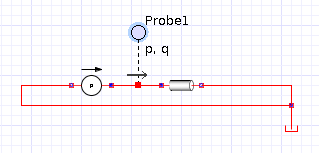
\includegraphics[width=0.5\textwidth]{img/simple-pipe.png}
\end{figure}
\begin{figure}[ht]
  \caption{Maplesim simulation of a simple rectangular pipe}
  \centering
    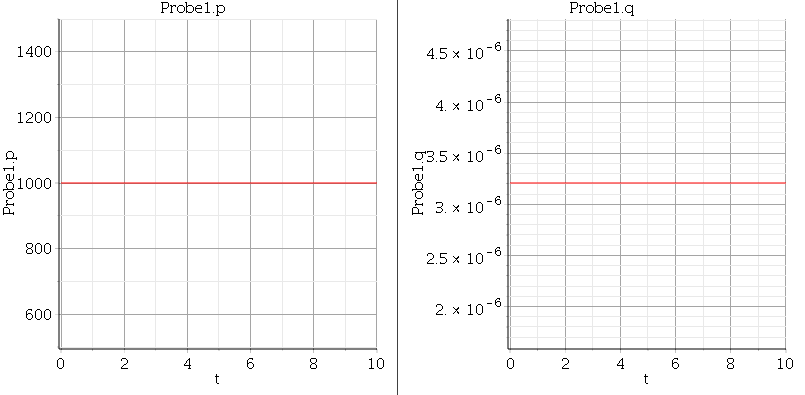
\includegraphics[width=0.5\textwidth]{img/simple-pipe-simulation.png}
\end{figure}


Though this is a simple example and is outside the microfluidics domain, Manifold's existing Modelica code generation can easily generate code using different libraries and can easily cope with more complex systems.
This example is a proof-of-concept demonstrating that Manifold frontend code can be used to generate Modelica models and then MapleSim graphs.

\section{Related Work}



\section{Future Work}

\subsection{Manifold Language}

Microfluidic circuit often have identical components that are used repeatedly.
We would like to add looping constructs to Manifold, either by creating a
macro system or by creating new builtin Manifold functions. A looping function
can take a component as a parameter and then repeat an action on that
component a number of times, such as connecting them to another component.
This feature in Manifold would not only save the programming from repeating
code, it also allows a programmer's design to scale up to a number of
components that would not be feasible to write by hand. We intend for
programmers to also be able to specifying size parameters for components as
well, such as a T-junction with \emph{n} branches.

\subsection{CEGAR Loop}

The Manifold backend's toolchain flow has so far been entirely linear.
The backend first generates SMT2 code for dReal and dReal gives it a basic first test of the system's viability.
Once dReal finishes, its outputs are parsed, inferred variables are filled in when needed, and a Modelica model is generated for MapleSim.
dReal and MapleSim run in a linear sequence and never run more than once.

One way to extend this flow is to turn it into a loop.
Not only would dReal output help generate inputs for MapleSim, but MapleSim would help generate new inputs for dReal.
The first and simpler half of the loop is already part of the original linear flow.
By interpreting MapleSim's outputs, the Manifold backend can determine how successful the simulation was relative to the engineer's expectations.
Based on these results, the backend would revisit the systems of SMT2 equations it generated earlier.
New values from within dReal's output ranges could be chosen for the next MapleSim generation.
Another option is to constrain the values of inferred values into smaller ranges based on the results and run dReal again on an increasingly constrained system.

CEGAR stands for counterexample-guided abstraction refinement.
The principle is that certain systems fail a satisfiability test or simulation, the failed system serves as an example of what not to do.
The counterexample allows the plausible ranges for certain variables to be reduced.
Given enough runs of a CEGAR loop, the ranges of inferred variables can be narrowed.
Over time, the design ends up more refined.

% Define block styles
\tikzstyle{decision} = [diamond, draw, fill=blue!20, 
    text width=4.5em, text badly centered, node distance=3cm, inner sep=0pt]
\tikzstyle{block} = [rectangle, draw, fill=blue!20, 
    text width=5em, text centered, rounded corners, minimum height=4em]
\tikzstyle{line} = [draw, -latex']
\tikzstyle{cloud} = [draw, ellipse,fill=red!20, node distance=3cm,
    minimum height=2em]

\begin{figure}[!ht]
\label{fig:cegarloop}
\caption{The Manifold toolchain with a CEGAR loop}
\begin{tikzpicture}[node distance = 2cm, auto]
    % Place nodes
	\node [cloud] (start) {Begin Design};
    \node [block, below of=start] (code) {Write Code};
    \node [block, right of=code, node distance=3cm](compile) {Compile the Code};
    \node [decision, below of=compile](dcompile) {Successful Compilation?};
	\node [block, right of=dcompile, node distance=3cm](smt2_codegen){Generate SMT2};
	\node [block, below of=smt2_codegen, node distance=3cm](dreal){DReal};
	\node [decision, left of=dreal](dDReal){attribute assignment found?};
	\node [block, below of=dDReal, node distance=3cm] (modelica_codegen) {Generate Modelica};
	\node [block, below of=modelica_codegen](MapleSim) {MapleSim};
	\node [decision, below of=MapleSim](dpass_sim){Pass Simulation?};
	\node [cloud, below of=dpass_sim](end){Design Complete};
	\node [block, right of=modelica_codegen, node distance=3cm] (refine){Refine Constraints};

    % Draw edges
    \path [line] (start) -- (code);
    \path [line] (code) -- (compile);
    \path [line] (compile) -- (dcompile);
    \path [line] (dcompile) -| node[near start]{no} (code);
    \path [line] (dcompile) -- node[near start]{yes} (smt2_codegen);
    \path [line] (smt2_codegen) -- (dreal);
    \path [line] (dreal) -- (dDReal);
    \path [line] (dDReal) -| node[near start]{no}(code);
    \path [line] (dDReal) -- node[near start]{yes}(modelica_codegen);
    \path [line] (modelica_codegen) -- (MapleSim);
    \path [line] (MapleSim) -- (dpass_sim);
    \path [line] (dpass_sim) -- node[near start]{yes} (end);
    \path [line] (dpass_sim) -| node[near start]{no} (refine);
	\path [line] (refine) -- (dreal);
\end{tikzpicture}
\end{figure}

\subsection{COMSOL Code Generation}

COMSOL Multiphysics (``COMSOL") is a powerful and proprietary simulator and finite element analyzer.
It supports add-ons for a wide variety of domains, including fluid mechanics.
We are interested in applying COMSOL because it promises a more deep and thorough simulation of the microfluidic devices than what MapleSim is capable of.
COMSOL has a Java API, so it should be possible to integrate it into Manifold's existing Java codebase and have it be called automatically.

% TODO: more about how COMSOL actually works and its value proposition.

We would like to add COMSOL to the CEGAR loop described above.
COMSOL is much slower and much more thorough than dReal or MapleSim, so it would not be in the main analysis loop.
COMSOL is best placed at the end of the analysis process, once the initial backend loop is confident in the design.
A COMSOL run would be the last step in the verification process and a successful run would indicate a high degree of confidence in the design.

We have refrained from trying to integrate with COMSOL so far, mainly due to COMSOL's complexity and steep learning curve.
However, COMSOL integration would bring significant power and mathematical rigour to the Manifold toolchain.

\section{Acknowledgments}



\section{Conclusion}





% disabling macros that are used only for UW Faculty of Engineering reports
\providecommand{\StudentAuthor}{}
\providecommand{\PostDocAuthor}{}
\bibliographystyle{IEEEtranN}
\bibliography{IEEEabrv,bib/strings-long,main,bib/microfluidics,bib/derek,bib/proceedings}


\end{document}
